\documentclass{article}
\usepackage{graphicx}

\title{My first latex tutorial}
\author{Charles León}

\begin{document}
	\maketitle
	\begin{abstract}
		Bueno, empezaré a escribir en latex porque al parecer es the best.
		Sin embargo, me preocupa, y bastante, que tenga que pelearme con los símbolos aquí. Las tildes van a ser un dolor de cabeza, ya lo vi. Also, esto no es un abstract
	\end{abstract}

	
	\section{Instalación (aka las previas)}
		
	Bueno, antes de empezar siquiera a tratar de escribir con un formato decente, el cómo instalé LaTeX y conseguí que funcionara se debe a dos fuentes:
	
		LaTeX for everyone and everything (Safari Books)
		
		How to Install Latex for Windows (https://www.youtube.com/watch?v=PMKRNl5w3DQ)
	
	Installé el MikTex como distribuidor de LaTeX y lo agregué manualmente al path (hay que buscar el bin en los archivos de programas). En el curso recomiendan montar un ISO de 2GB, por lo que busqué otra alternativa que no sé si será mejor a largo plazo. En el video de YouTube recomendaban TexMaker, pero nunca logré que compilara algo. En el curso recomiendan TeXstudio, y este me ha funcionado bastante bien.
	
	Por cierto, intenté seguir el curso LaTeX A-Z, pero no hicimos click
	
	\section{Primer experimento}
	
	Si le doy a Tools->Build and View cuando todo el documento está en blanco sale un error en la consola. Si solo pongo la cabecera documentclass también sale un error. Es necesario un begin y end para que recién el artículo pueda compilar. Borrar la cabecera también da error.
	
	\section{Getting Started and Basic Documents (Chapter 2)}
	
	\subsection{Creating our First Document}
	
	Diferencias entre editor y distribución (compilador)
	
	TexStudio -- Editor (source code)
	
	TeXLive -- Compiler --> PDF (supongo que en este caso sería miktex)
	
	En este enlace hay una explicación sobre MiKTeX y TeX Live
	
	 (https://www.texdev.net/2016/12/18/tex-on-windows-tex-live-versus-miktex-revisited/)
	
	Commands - empiezan con el backslash
	
	Command table documentclass - hay bastantes, pero empezaremos con el article red
	begin - document blue
	end - blue
			title - wow red
			author - wow red
			maketitle - this one blew my mind, pero lo de la fecha, eh red
			
	La zona entre el begin y el end se llama Document environment, y la zona entre el documentclass y el begin Preamble (wikibooks latex document structure)
	
	\subsection{Basic Document Structure}
	
	Command table ...
	documentclass book
	section
	subsection
	subsubsection (it apperas this to be the limit)
	label sec fig no idea what's this for
	
	\section{Introduction}
	This is going to be a normal paragraph.
	\subsection{Some Background}
	And some more text here
	\subsubsection{Drilled Down}\label{sec:drilled-down}
	More text.		
	Con documentclass book, la seccion tendría otro sistema de numeración
	
	shortcuts ctrl k borra una linea (discovered by me)
	
	begin abstract
	
	¿Por qué hay comandos azules y rojos?
	\newpage
	\subsection{Inserting Figures (and Best Practices)}
	
	command
	newpage
	includegraphics is in a package width ata thte begininng
	textwidth
	figure environment
	packages
		graphicx
	begin figure to the top optional parameter
	label fig
	
	\begin{figure}
	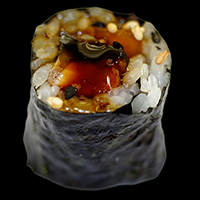
\includegraphics[width=1\textwidth]{makis}
	\caption{jum}\label{fig:first-figure}
	\end{figure}
	jum
	es una buena practica ponerlo o suber arriba o super abajo
	
	\subsection{Inserting Tables}
	
\end{document}